\section{Introduction}

% LaTeX intro
When researchers hope to begin drafting a thesis, chapter, report, or a paper, they frequently lean toward using \LaTeX, which is a typesetting system that is commonly used to prepare technical and scientific documents \cite{latex}.
\LaTeX\ separates the authors' contents from the formatting requirements.
This allows publishers and editors to alter or enforce consistency in formatting without interacting with the textual content of the documents.

% LaTeX efficiency study results
While \LaTeX\ eases the editorial process for the publishers, it requires authors to learn its syntax and semantics.
While an experienced \LaTeX\ user may be more efficient in drafting their documents, the same is not observed among first-time or one-time users.
Studies identify that \LaTeX\ is particularly powerful in rendering mathematical expressions and equations, which is identified by experienced and inexperienced users alike and is exploited for higher efficency \cite{knauff_efficiency_2014}.
Common general-purpose document processing software like Microsoft Word, Google Docs, and LibreOffice recognise the same, and allow authors to embed a snippet of \LaTeX\ code to render mathematical sections within documents authored on their platforms \cite{matthews_craft_2019}.
However, rendering a table using the language is highly tricky to get right due to the complicated syntax, and even experts regularly struggle with this task \cite{knauff_efficiency_2014}.

% Solutions to generate LaTeX
The complexity of the \LaTeX\ syntax can be attributed to the extent of detail and complexity it affords, but the consequence is that rendering a basic component also becomes difficult.
For this purpose, researchers look towards ways to simplify the process of writing \LaTeX\ code.
Echoing the trickiness of creating tables in \LaTeX, Kayal et al. built a system to recognize tables using OCR and and render tables using a ResNet transformer \cite{kayal_tables_2023}.
A similar solution was explored by Xia et al. to convert images and tables to \LaTeX\ compatible code \cite{xia_latexnet_2025}, which collects images and tables along with their corresponding \LaTeX\ code from the preprint repository ArXiv and trains an image multiplexer convolutional neural network.
They observed high similarity across the generated and expected code.

% Generative AI bad in academia
The surge in large language models (LLMs) and generative artificial intelligence (GenAI) sees widespread adpotion in fields like creative work, software development, data analysis, and so on.
However, students and researchers in academia are strongly advised against using GenAI for their work.
Studies show heightened usage of LLMs across research publications, and attribute it with lowered quality of material, increase in communication inaccuracy, and an abnormal shift in the language and vocabulary \cite{kobak_delving_2025}.
For these reasons and more, surveys reveal that GenAI usage is generally shunned upon by adacemia \cite{kwon_survey_2025}.
Although scholars in STEM-based fields are more welcoming of GenAI as a tool whose usage may be accepted with responsible disclosure, scholars in non-STEM fields are more strictly against the usage of GenAI in their literature.

% Maybe GenAI not so bad?
As a result, scholars miss out on the productivity boost that GenAI can offer.
With a purpose-built tool that respects the ethical considerations that the academic community has, students, researchers, and publishers can benefit from a lot of the day-to-day issues that tend to slow down the research and publication process.

% Spartan Write!
This report introduces Spartan Write, an AI-powered document authoring platform designed for scholars and researchers preparing academic reports, articles, papers, and theses.
At its core, Spartan Write pairs an intelligent agent with \LaTeX, enabling users to draft, edit, and refine documents through natural conversation.
The agent assists with generating sections, structuring tables, managing figure placement and captions, and handling LaTeX formatting, all without requiring users to write raw markup.
To ensure consistency and reduce formatting overhead, Spartan Write provides curated document templates spanning common academic genres.
The result is a seamless blend of conversational AI and professional typesetting, letting researchers focus on content rather than technical details.

\begin{figure}[htbp]
    \centering
    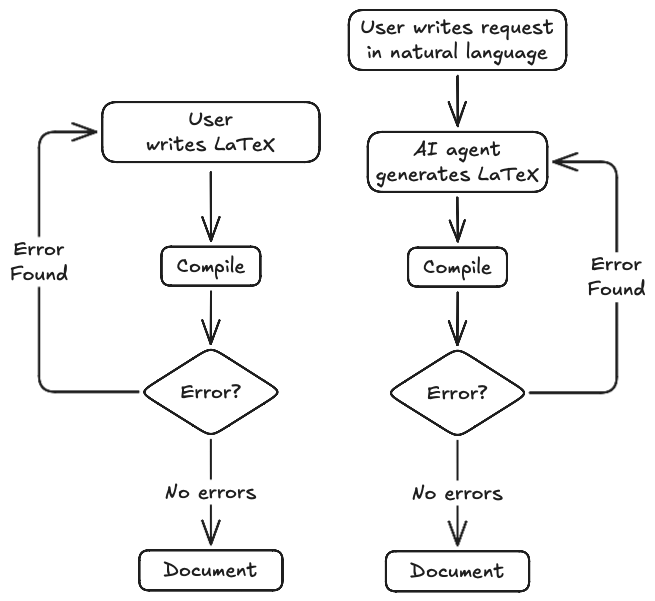
\includegraphics[width=.9\linewidth]{figures/authoring-workflow.excalidraw.png}
    \caption{A comparison of authoring workflows using \LaTeX\ (left) and using Spartan Write (right)}
    \label{fig:authoring-workflow}
\end{figure}
